\section{Thesis Proposal}
\label{sec:proposal}

The formal understanding of early warning signals of critical transitions requires future clarification; specifically, the current theory relies on long-term and linear approximations while ignoring transient behavior. 

One line of research seeks to clarify the effect of short term non-exponential behavior. For example, reactivity has recently been shown to change systematically leading up to bifurcation in a certain class of infectious disease models \cite{oreganTransientIndicatorsTipping2020}. 

On the other hand, I propose to clarify the effect of behavior far away from the attractor -- far enough that it is not within the descriptive bounds of a linear approximation. I suggest investigating the relationship between intensity of attraction and critical transitions. 
%
Toward this goal, I propose to relate intensity to at least two different types of tipping behavior: local bifurcations, and tipping across basin boundaries. As a supplementary pursuit, I would also like to improve the general theoretical understanding of intensity of attraction, by considering assorted open questions related to it. 
%Finally, I will mention at the end of this section some further possible connections -- to machine learning based warning signals and a framework known as  flow-kick systems. 
%
Perhaps this work can help build toward an eventual theory of early warning indicators brought about by changes in intensity before a critical transition. 

\todo{note: from here onward the draft is in a less well-organized/ complete form.}

%I would like to pursue analytic results as well as application-specific examples. 

%Propose some avenues that may help build toward a theory of early warning indicators brought about by changes in intensity during the time leading up to a critical transition. 
%
%Might be that intensity only provides useful warning indicators in a specific class of critical transitions, or for a specific class of ODEs. 

TO DO: Motivating example where intensity might be useful. (I have not constructed this example yet.)

%\subsection{Continuity of Intensity}

%\subsection{Demographic Versus Environmental Perturbations}

\subsection{Intensity Through Local Bifurcations}

How does intensity of attraction behave when passing through a local bifurcation? Does it display a systematic change, similar to the way that asymptotic resilience? 

%Why does this matter? Connect back to motivation. 

Here, a first step may be to prove continuity (or a weaker version of continuity) of intensity with respect to parameter changes. 

\begin{conjecture}(McGehee)
	Intensity is continuous (or upper semi continuous?) with respect to parameter changes. To do: phrase this formally. What is the right way to do this? Kate says Dick conjectured this during her thesis defense. The attractor itself is upper semi-continuous. 
\end{conjecture}

Next, I would investigate one dimensional saddle-node, transcritical, and pitchfork bifurcations. 
%
Start with numerical computations of intensity across application-specific examples of bifurcation, or maybe using normal forms of bifurcations. Then try to prove analytic results. 
%
I think in these bifurcation types, intensity should go to zero. In some systems intensity may decrease at a similar or proportional rate as does asymptotic resilience. But in others, their two rates of decrease may not be as straightforwardly related. Maybe some kind of object measuring the relatedness between the two could be defined. What would that mean?

%Why do I think this? Provide justification.

%Some authors have argued that another basin-based measure of resilience, basin-width, is linearly related to asymptotic resilience -- to do: cite and check if the phrasing is correct. 

Hopf bifurcations. Could start with Kate's Lotka-Volterra example and do a numerical simulation at the bifurcation value to see what intensity looks like there. Here the point attractor disappears, but, replacing it with the new periodic orbit as the attractor of interest, intensity should be continuous through the bifurcation?  %Not really sure what to expect here in general. 

%Maybe nothing interesting?

Another idea: "\textbf{Critical Widening}". What I mean:

Critical slowing down is usually thought of as a response to state variable perturbations, where the perturbation is drawn from some fixed random distribution. In particular, the size of perturbations shouldn't change over time, only the rate of recovery from them. 

However, in empirical examples, the size of perturbations tends to also increase close to bifurcation. For example, increased variance manifests with slowing down (points take longer to go back to the mean) but also widening (points go farther away from the mean in the first place).  (Like in Figure \ref{fig:csd}, where the second variance graph looks as though it is stretched longer horizontally but also wider vertically, compared to the first variance graph.)

So to me this says 2 things:

1) Modeling perturbation as something drawn from a fixed distribution and added to the state variable is not quite right. Instead, perturbation should also be modeled as something added to the vector field -- a la Kate and intensity. In Tiffany's class, I learned a name for these two types of perturbations: demographic (state variable) vs. environmental (vector field), and in reality systems can face some combination of both.

2) The fact that perturbations get wider near bifurcation is implicitly because: basin steepness is decreasing (intensity is going down). Because that way, the same vector field perturbation pushes you a farther distance than before. 

So maybe the widening phenomenon needs to be separated from the slowing down phenomenon. When looking at data, you shouldn't just check if there's increased variance, but check how much increased variance of each type (widening and slowing down types). Because each informs you about a different type of resilience, and maybe you expect in your system for asymptotic resilience to change in a certain systematic way and intensity of attraction to change in some other systematic way. You could be more confident about the reliability of your early warning signal this way.

Does this thought about critical widening make any sense? Should I try to write it up better to include in the final version of this section?

%For example, increased variance of the slowing down type tells you about resilience to demographic perturbations. While increased variance of the widening type tells you about resilience to vector field perturbations. 

%I feel like right now both are just swallowed into the term critical slowing down. 

%Not explained by critical slowing down with state variable perturbation. But can be explained by decreasing intensity leading up to bifurcation with vector field perturbation. In reality perturbations may be a combination of state and vector field perturbations (e.g. demographic and environmental perturbations).

\subsection{Tipping Across Basin Boundaries}

Critical slowing down is usually thought of in relation to one specific category of tipping behavior – local bifurcations. But another class of tipping behavior occurs when perturbations push a state variable into an alternative basin of attraction. Intensity measures how difficult it is for this type of tipping to occur. (Many other dynamical behaviors also correspond to tipping, and are not considered here, including global bifurcations, rate-induced tipping, and transitions to chaotic regimes.)

Mention flickering and/or skewness indicators. But these are also understood from an informal point of view, with unclear formal basis. 

There ought to be a formal basis for a theory of early warning signals for basin boundary tipping -- and maybe intensity is a good framework to build it in.

\subsubsection{Reversibility of Hysteretic Transitions}

Hysteresis is a phenomenon used to describe transitions which are not immediately reversible. Suppose you increased a parameter value, causing your system to tip over a saddle-node bifurcation to a new attractor. Simply decreasing the parameter back to the original value may not be enough to tip it back to the old attractor -- you might need to decrease it much more in order to achieve reversal. Figure (\ref{fig:hysteresis}).

\begin{figure}[ht]
	\centering
	\captionsetup{width=0.4\linewidth}
	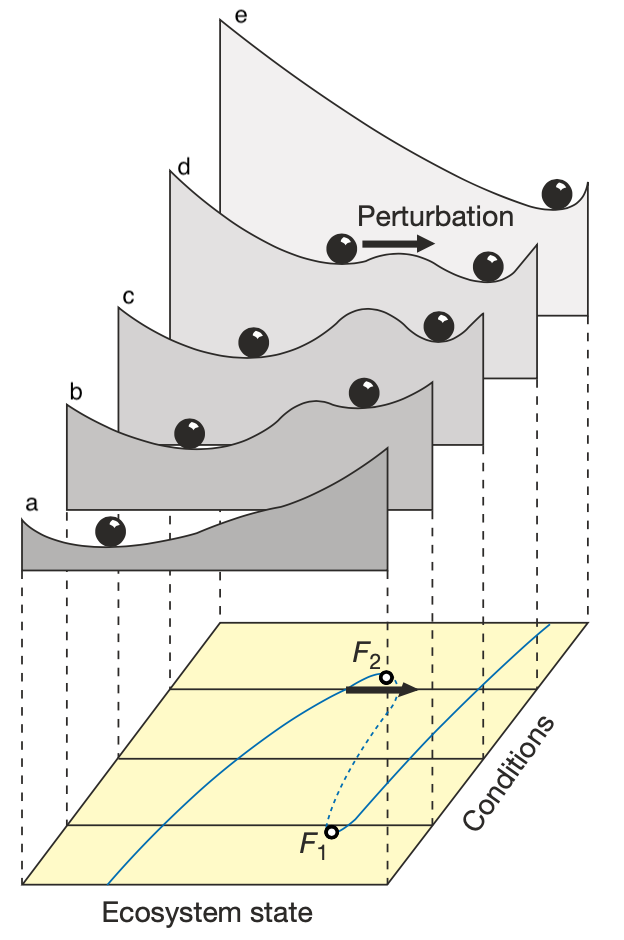
\includegraphics[width=0.4\textwidth]{figs/hysteresis}
	\caption{Hysteresis. Figure reproduced from \cite{schefferCatastrophicShiftsEcosystems2001a}.}
	
	\label{fig:hysteresis}
\end{figure} 

%At least two types: cubic type or parabolic plus additional steady state type (e.g. KIausmeier equation)

However, in a noisy system, you might not need to work quite as hard to achieve reversal -- a perturbation could push you back into the other basin of attraction prematurely. So there's some chance you can bypass some of the hysteresis and restore your old state sooner. How do you know if this is likely to happen?

Intensity of the two alternative attractors helps describe how easy it is to switch to the other attractor. So maybe intensity can help give a measure of how hysteretic a bifurcation really is -- from completely hysteretic to easily reversible.

Also, is it useful to define an intensity for the repeller in between the alternative attractors?

\subsection{General Open Questions About Intensity}

\subsubsection{Estimates of Intensity}
One basic limitation of using intensity of attraction in any application right now: numerical computations of intensity (which currently use set-valued Euler methods on a fixed grid) are too time-intensive. Instead, analytic tools should be developed that can be used for estimating intensity. (There is also a need for improved numerical methods, although this important avenue is not the focus of my thesis proposal.) A proof of Conjecture \ref{conj:steepness} could provide a useful way to estimate lower bounds on intensity that doesn't require full numerical computation. 

\subsubsection{Critical Reachable Set}

What is the smallest set $A \subset N \subset basin(A)$ so that if $N \subset R_r(A)$ then $intensity(A) \leq r$?

In other words, if under $r$-bounded control you can reach $N$ then you can escape the basin. This is a critical set in the sense that it is the "hardest" part of the basin to overcome -- once you can reach $N$ then you can leave the basin. 

\subsection{Further Possibilities}

Machine learning based early warning signals? %Possible connection between machine-learning based and analytical theory based early warning signals? i.e. using theory to inform ML design. 
This is something cool and related, which I learned about in Math Bio class. 

%Validating on actual data from somewhere?

Connections to Multiflows?

Connections to Flow-Kick systems? 

